\documentclass[11pt,english]{article}
\usepackage[latin9]{inputenc}
\usepackage{geometry}
\usepackage{subfig}	%%for easy placement of multiple pictures inside one figure
\geometry{verbose,letterpaper,tmargin=1in,bmargin=1in,lmargin=1.3in,rmargin=1.3in}
\usepackage{graphicx}
\usepackage{amssymb}
\usepackage{pdfpages}
\usepackage{hyperref}
\makeatletter

%%%%%%%%%%%%%%%%%%%%%%%%%%%%%% LyX specific LaTeX commands.
\newcommand{\noun}[1]{\textsc{#1}}
%% Bold symbol macro for standard LaTeX users
\providecommand{\boldsymbol}[1]{\mbox{\boldmath $#1$}}

%%%%%%%%%%%%%%%%%%%%%%%%%%%%%% User specified LaTeX commands.
\usepackage{color,calc}
\definecolor{shade}{gray}{0.984}
\newenvironment{myFramedBox}[1][]%
        {
        %\setlength{\fboxsep}{-\fboxrule}
        % \footnotesize\normalfont\ttfamily\raggedright
        \setlength{\rightmargin}{\leftmargin}
        \setlength{\itemsep}{-12pt}
        \setlength{\parsep}{20pt}
        \begin{lrbox}{\@tempboxa}%
        \begin{minipage}{\linewidth-2\fboxsep}
        }%
        {
        \end{minipage}%
        \end{lrbox}%
        \fcolorbox{black}{shade}{\usebox{\@tempboxa}}\newline\newline
        }%

\usepackage{babel}
\makeatother

\setlength{\textwidth}{6.50in}      % was 6.00
\setlength{\evensidemargin}{0.05in} % was 0.25
\setlength{\oddsidemargin}{0.05in}  % was 0.25
\setlength{\textheight}{8.80in}     % was 8.5 or 9.0
\setlength{\topmargin}{-0.7in}      % was -0.5
\setlength{\parskip}{2.0mm}         % was 2
\setlength{\baselineskip}{1.7\baselineskip}

\newtheorem{theorem}{Theorem}
\newtheorem{lemma}[theorem]{Lemma}
\newenvironment{proof}{{\noindent \em Proof:~}}{\hfill{\hfill$\Box$}}

\newcommand{\complexityclass}[1]{{\bf #1}}
\newcommand{\NP}{\complexityclass{NP}}
\newcommand{\RE}{\complexityclass{RE}}

\begin{document}

%\def\thepage{}

\title{Elliptic Curve Cryptography\\Final report for a project in computer security}


\author{
   Gadi Aleksandrowicz\thanks{
      Dept.\ of Computer Science,
      The Technion---Israel Institute of Technology,
      Haifa~32000, Israel.
      E-mail: {\tt gadial@cs.technion.ac.il}
   } \and
   Basil Hess\thanks{
      Dept.\ of Computer Science,
      ETH Zurich,
      8092 Zurich, Switzerland.
      E-mail: {\tt bhess@ethz.ch}. Work done while visiting Technion.
   }
}

\date{}

\maketitle

\section{Introduction}
An \emph{Elliptic Curve} can be roughly described as the set of solutions to an equation of the form $y^2=x^3+ax+b$ over some field (e.g. $\mathbb{C}, 
\mathbb{R},\mathbb{Q}$ or some finite field $\mathbb{F}_{p^n}$). The importence of elliptic curves stems from their rich structure: there is a rather simple
addition law definable on elliptic curves which makes them into an abelian group. Studying the emerging structure of elliptic curves over various fields has been a
major theme in the mathematics of the 20th centaury, and elliptic curves were connected to many famous problems and results, most notably the proof of Fermat's
last theorem\marginpar{Give some reference, to a good survey if possible}.

In the late 70's, \emph{Public-Key Cryptography} systems were first publicly described, changing the face of cryptography. Many of the purposed systems, such
as the Diffie-Hellman key exchange system and the ElGamal encryption system\marginpar{Reference to both papers}, were based on arithmetic in the group $\mathbb{Z}_p$, but in theory could
be implemented in other groups as well. Groups based on elliptic curves were a good choice because of their well-developed theory and their high variety. In 1985,
both Neal Koblitz and Victor S. Miller \marginpar{Ref...} suggested public key cryptosystems based on elliptic curves.

Our goal in the project has been to implement an efficient public key cryptosystem based on elliptic curves ``from scratch'', relying only on large-number arithmetic
libraries. In particular, we have implemented all the elliptic-curve related calculations, and additional related algorithms.

\section{Elliptic Curves}
\subsection{Definition}
Most generally, and elliptic curve $E$ over a field $K$ can be described as the subset of $K\times K$ satisfying the equation $$y^2+a_1xy+a_3y=x^3+a_2x^2+a_4x+a_6$$ 
for a given $a_1,a_2,a_3,a_4,a_5,a_6\in K$, along with another special point ``at infinity'' $\mathcal{O}$. An additional demand is that the curve be ``smooth'',
which means that the partial derivatives of the curve has no common zeros. This can be reduced to checking that some invariant value $\Delta$ (the \emph{discriminant} of the curve)
which is calculated from the coefficients is not zero\marginpar{Add a picture}. Because the nature of the field $K$ is highly relevant to the structure of $E$,
it is common to write $E/K$ indicating the curve $E$ (usually given by the equation) iis defined over the field $K$.

Depending on the characteristic of $K$, the above equation can be simplified. There are three cases to consider:
\begin{enumerate}
  \item When $charK\ne 2,3$ the equation can be simplified to $y^2=x^3+ax+b$ with $a,b\in K$.
  \item When $charK = 2$ and $a_1 \ne 0$, the equation can be simplified to $y^2+xy=x^3+ax^2+b$ with $a,b\in K$. This curve is said to be \emph{non-supersingular}. If $a_1 = 0$, the equation can be simplified to $y^2+cy=x^3+ax+b$ with $a,b,c\in K$. This curve is said to be \emph{supersingular}.
  \item When $charK = 3$ and $a_1^2\ne -a_2$, the equation can be simplified to $y^2=x^3+ax^2+b$ with $a,b\in K$. This curve is said to be \emph{non-supersingular}. If $a_1^2=-a_2$, the equation can be simplified to $y^2=x^3+ax+b$ with $a,b\in K$. This curve is said to be \emph{supsersingular}.
\end{enumerate}

\subsection{Motivating Example: $K=\mathbb{C}$}
A \emph{lattice} in the complex plane $\mathbb{C}$ is a set of the form $L=\{n\omega_1+m\omega_2|n,m\in\mathbb{Z}\}$ such that $\omega_1,\omega_2\in\mathbb{C}$ are
not colinear. Lattices can be used to generalize the notion of ``periodic function'' to the complex plane: A meromorphic function $f$ is called \emph{elliptic} with respect to the lattice
$L$ if $f(z+l)=f(z)$ for all $l\in L$ (equivalently, $f(z+\omega_1)=f(z+\omega_2)=f(z)$). Thus it suffices to know the values of $f$ of the \emph{fundemental parallelogram} $\Pi=\{a\omega_1+b\omega_2|a,b\in[0,1]\}$
in order to know its values on the complex plane.

In $\mathbb{R}$, the periodic function $\sin(x)$ is ``special'' in the sense that along with its derivative, $\cos(x)$. it can be used to represent all
the periodic functions (via Fourier series). There is a parallel ``special'' function for elliptic functions, which in some regards is ``even better'' than its real counterpart. 
Given a lattice $L$, the \emph{Weierstrass $\wp$-function} for this lattice is defined as $$\wp(z)=\frac{1}{z^2}\sum_{0\ne l\in L}\left(\frac{1}{(z-l)^2}-\frac{1}{l^2}\right)$$
$\wp$ has the property that every elliptic function (in respect to a given lattice $L$) can be written as a \emph{rational} function in $\wp$ and $\wp'$ (as opposed to the
infinite sum of $\sin$ and $\cos$). Thus $\wp$ is the most significant example of an elliptic function.

Let $E/\mathbb{C}$ be an elliptic curve given by $y^2=x^3+ax+b$. A lattice $L$ can be found such that the corresponding Weierstrass function satisfies the differential equation
$(\wp')^2=\wp^3+a\wp+b$. This means that the map $z\mapsto (\wp(z),\wp'(z))$ maps $\mathbb{C}$ to points on the elliptic curve. In particular, $\wp$
has a pole in each lattice point and so $0\mapsto \mathcal{O}$ (this can be made precise by using projective coordinates). Moreover, it
can be shown that this map is onto, and that $z_1,z_2$ give the same point on the curve if and only if $z_1-z_2\in L$, and so we have a bijection
between $E$  and $\mathbb{C}/L$, the latter set can be thought of as a torus (since $\mathbb{C}/L$ is isomorphic to $\Pi$ where parallel edges are ``glued`` together).

Since $\mathbb{C}/L$ can be equipped with an operation of addition modulu $L$, it forms an abelian group. This group structure can thus be induced on the 
isomorphic elliptic curve: Given $P_1, P_2$ on the curve that emerge from $z_1,z_2$ (i.e. $P_i=(\wp(z_i),\wp'(z_i))$) we define $P_1+P_2=(\wp(z_1+z_2),\wp'(z_1+z_2))$ 
(with the addition of $z_1+z_2$ done modulu $L$). This shown that every elliptic curve over $\mathbb{C}$ is an abelian group.
\subsection{The Group Operation}
In the previous section we have seen how eliiptic curves over $\mathbb{C}$ can be naturally induced with a group operation. There is no similar theory over
other fields, but we can still axiomatically define an operation similar to the one arising in the complex case. A detailed analysis of the complex case yields
the following rough description of the group operation:

First, for the special point $\mathcal{O}$ we have $P+\mathcal{O}=\mathcal{O}+P=P$, so $\mathcal{O}$ is the identity element.

Second, $(x,y)+(x,-y)=\mathcal{O}$ (note that if $(x,y)\in E$ so is $(x,-y)$ since the in equation defining $E$ is of the form $y^2=x^3+ax+b$ and so for
every $x$ we have two possible values of $y$, given that $x^3+ax+b$ has roots at all). So given a point $P$, its additive inverse $-P$ is simply the same point
with the sign of the y-coordinate flipped.

Third, for every three colinear points on the curve $P,Q,R$ we have $P+Q+R=0$, and so $P+Q=-R$. We can picture this in the following manner: Given $P,Q$,
to compute their sum draw a line passing through them, and find the third point where the line crosses the curve (there is always such one - if it seems the line 
''misses`` the curve, it actaully intersects it in $\mathcal{O}$; again, using projective coordinates this can be made precise). After such a point was found, we
take its inverse to be the result of $P+Q$. This might seem like an arbitrary definition, and so it is worthwhile to remember that it is actually a result of the non-arbitrary
operation induced in $\mathbb{C}$.

We also need to describe what is $P+P$. In this case we cannot pass a single line ''between $P$ and itself``, but we have a similar notion: Since the curve is smooth,
it has exactly one tangent line in each point. Therefore we have that $P+P$ is the additive inverse of the point of intersection with the curve of the tangent line to the curve at $P$.

This completes the description of the group operation. Although it arises from the complex case, this description is valid over any field, and can be taken to be
the definition of the group action. In is a straightforward technical manner to check that the axioms for group operation are indeed satisfied by this operation.

The geometrical description of the operation is insightful but of little use in algebraic calculations. However, straightforward analytic geometry
gives simple equations for calculating addition of points. The actual equations depends on the simplified form of the curve; we will focus later on the cases
where $charK\ne 2,3$ and $charK=2$ as these are the main cases used in practice.

\subsection{Group Structure}
The structure of the group of an elliptic curve highly depends on the underlying field. For $K=\mathbb{C}$ we have already seen that it has the structure of a torus.
Over $\mathbb{Q}$, a famous theorem of Mordell shows that the group is finitely generated; since it is also abelian, it is of the form $\mathbb{Z}^r\times Z$
where $Z$ (the \emph{torsion} subgroup of the curve) is a finite abelian group. The torsion of an elliptic curve is easy to compute and is very well known -
it is known that there are only 15 possible torsion subgroups, the largest of whom of cardinality 16. The main difficulty is computing the parameter
$r$ - the \emph{rank} of the curve. Of the the most famous open conjectures in mathematics, the Birch and Swinnerton-Dyer conjecture, deals
with the connection between the rank of a curve (and various other related parameters) and the behivour of a special function related to the curve (the
zeta-function of that curve).

Over a finite field $K=\mathbb{F}_q$ ($q$ a power of a prime), the order of the curve is, of course, finite. However, it is not easy to know in general
what is the exact number of points on the curve.  A reasonable estimate is given by Hasse's theorem, which shows that the order is roughly $q+1$, with
a square-root bound on the error. More precisely, if $\#E(\mathbb{F}_q)$ is the number of points on the curve $E$ over $\mathbb{F}_q$, then 
$|\#E(\mathbb{F}_q)-(q+1)|\le 2\sqrt{q}$

Knowing the order of the curve is very important when using curves for cryptographic purposes. There exist algorithms for computing the order, but
they are quite complicated and not very efficient. Thus, sometimes a different approach is used - first the order is chosen, and then a suitable curve
for that order is generated. We elaborate on this later.
\section{Elliptic Curve Arithmetic}
\subsection{Projective Coordinates}
As we shall see, the usual usage of elliptic curve in cryptosystems is in computing $P+P+\dots+P$ for a given point $P$. 
The formulas for adding points on the curve includes a division operation, which in most implementations is very costly. Therefore, it is reasonable to
transform the coordinate system into one in which no division is needed for the addition operation itself, only for transforming back to the standard
coordinate system once the calculation is complete. Such a coordinate system is the \emph{projective} coordinate system.

Theoretically it is possible to imagine the projective coordinate system as one in which every two-dimensional point is represented by a ray in the three
dimensional space. Formally we consider the set $K^3\\\{(0,0,0)\}$ with an equivalence relation charctarisied by two positive integers $c,d$ and
defined by $(X_1,Y_1,Z_1)\sim (X_2,Y_2,Z_2)$ if $X_1=\lambda^cX_2,Y_1=\lambda^dY_2,Z_1=\lambda Z_2$ for some $\lambda\in K^*$ (for $c=d=1$
indeed we have that each equivalance class is a line in $K^3$).

The two-dimensional point $(X,Y)$ can be identified with the projective point represented by $(X,Y,1)$, and so in general a projective point represented by
$(X,Y,Z)$ with $Z\ne 0$ corresponds to a standard point $(\frac{X}{Z^a},\frac{Y}{Z^b})$. However, projective points represented by $(X,Y,0)$
have no standard two-dimensional equivalent, and so are considered ''points in infinity``. Indeed, this is a way to formally represent $\mathcal{O}$.

\subsection{Addition Formulas - The Prime Field Case}
We consider now the case $K=\mathbb{F}_p$ for $p>3$ prime (however, for any $K$ such that $char K\ne 2,3$ our description is essentially the same).
In this case let $E$ be a curve defined by $y^2=x^3+ax+b$. Given two points on the curve $P=(x_1,y_1),Q=(x_2,y_2)$ we first consider the case $x_1\ne x_2$
(and so $P\ne\pm Q$). The line passing both in $P$ and $Q$ has slope $\frac{y_2-y_1}{x_2-x_1}$ and so its equation is $y=y_1+\left(\frac{y_2-y_1}{x_2-x_1}\right)(x-x_1)$.

\subsection{Addition Formulas - The Binary Field Case}
In the binary case $K=\mathbb{F}_2$, the curve $E$ is defined by $y^2+xy=x^3+ax^2+b$. First note that the negative of a point $S=(x,y)$ is defined as $-S=(x,x+y)$, and it can be checked that the point $-P$ indeed also lies on $E$.
For the two points $P=(x_1,y_1),Q=(x_2,y_2)$ (denote $P+Q=(x_3,y_3)$), the easiest cases are when $P=\infty$ or $Q=\infty$. By the group law, it holds that $P+\infty=P$ and $\infty+Q=Q$ in those case. In the case of $P=-Q$, the result is $P+Q=\infty$.

The remaining two cases are $P=Q$ and $P\ne Q$.

In the case $P=Q$, we need to double the coordinate, where $\lambda=x_1+\frac{y1}{x1}$ is the slope of the tangent, analogue to the prime case. As resulting x-coordinate one gets $x_3=a+\lambda^2+\lambda$.

In the case $P\ne Q$, the slope of the connecting line is $\frac{y_1+y_2}{x_1+x_2}$ (note that addition and subtraction is the same in binary field arithmetic). It holds that $x_3=a+\lambda^2+\lambda+x_2+x_1$ (in the case $P=Q$, $x_2+x_1=x_1+x_1=0$).

Finally in both cases the y-coordinate is computed as $y_3=(x_2+x_3)\lambda+x_3+y_2$. The overall algorithm derived from the formula requires 3 multipications (one is squaring), one multiplicative field inversion, and 9 or 6 additions. While the additions are very cheap operations, computing the inverse could be avoided by using projective coordinates as described before.

\subsection{Point Multiplication}
Scalar point multiplication is a frequently used operation in the cryptosystem we implemented and it is therefore of a big importance to implement this efficiently. We want to compute $kP=Q$ for a scalar $k$ and a point $P$. Using only addition, one could compute this as $\underbrace{P+...+P}_{k}$, with a complexity of $O(k)$. A better way is to use the additive equivalent of the \emph{square-and-multiply} algorithm. There, $k$ is processed bitwise. At each iteration, the result is doubled, and if the bit equals one, $P$ is added. Let $[k_{\log{k}},...,k_1]$ be the bit-representation of $k$, with $k_1$ as the least significant bit:

\begin{enumerate}
 \item $Q=\infty$
 \item for $i=1..\log{k}$:
 \item $Q=Q+Q$
 \item if $k_i=1$: $Q=Q+P$
\end{enumerate}

The complexity of this algorithm is $O(\log{k})$. There are some optimizations to this algorithm, most notably the replacement of the binary representation of $k$ with its \emph{non-adjacent form} which results in a shorter representation. 

\subsection{Binary Field Arithmetic}
The arithmetic in a prime field $\mathbb{F}_p$ is basically well-now; addition, and multiplication correspond to integer arithmetic modulo $p$. Finding the inverse can be done using the extended euclidean algorithm. Those operations are provided in the big integer library GMP we used. As an additional algorithm we had to implement the modular square root.

In the binary extension field $\mathbb{F}_{2^d}\cong \mathbb{F}_2(\theta)/m(\theta)$, the arithmetic is slightly different and we implemented it from scratch. One could alternativly use a library like \emph{NTL}.

Elements of the binary field are actually polynomials of degree $d$ with binary coefficients. And all operations in the polynomial basis are done modulo the reduction polynomial $m(\theta)$. For example the polynomial $\theta^4+\theta+1$ can be displayed as the bit-string $10011$. There is also the normal basis field representation which we will not treat because the more inefficient behavior of its arithmetic.

\paragraph{Addition/Subtraction}
Addition is the simplest operation and is computed as bitwise XOR: for $a,b\in \mathbb{F}_{2^d}$, $a+b=a\oplus b$.
\paragraph{Multiplication}
Multiplication of two elements $a$ and $b$ has alway to be done modulo $m$. Lopez and Dahab \cite{715867} present some efficient algorithms for this case. We implemented one which reminds of the square-and-multiply algorithm and could be called shift-and-add algorithm ($a$ is represented as $a_l,...,a_1$ and $b$ as $b_l,...,b_1$, let the result be $c$):
\begin{enumerate}
 \item $c=0$
 \item for $i=l,...,1$:
 \item shift $c$ one to the left ($c=c<<1$)
 \item if $a_i=1$: $c=c+b$;
 \item if the degree of $c$ exceeds $d$: $c=c+m$
\end{enumerate}
We note that in each iteration, $c$'s degree could be at most one degree to high, it can therefore be reduced by $m$ by just adding $m$ to $c$.

\paragraph{Inverse}
As we know the extended euclidean algorithm can be used to compute the multiplicative inverse in a finite field. This is also the case with binary fields. Suppose we want to compute the inverse of $a$ modulo the reduction polynomial $m$. We have $aa^{-1}\equiv_m 1$, reforming this we get $aa^{-1}-1=mx$ for arbitrary $x$. This can be reformed to $aa^{-1}-mx=1$, which is is exactly the setup for the euclidean algorithm, since $gcd(a,-m)=1$, and the algorithm can run on the inputs $a$ and $-m$ and deliveres as one output $a^{-1}$.

\paragraph{Quadratic Equations}
A frequent task is the computation of a y-coordinate for a given x-coordinate. Reviewing the equation $y^2+xy=x^3+ax^2+b$, the problem is reduced to a quadratic equation $y^2+a'y-b'=0$, which has either two or no solution. The solutions of this equation equation is equivalent to the solution of $y^2+y=c'$ with $c'=\frac{b'}{a'^2}$.

The procedure how to solve this equations is described in IEEE P1363/D13, and works as follows:
\begin{enumerate}
 \item Choose a random $\rho\in\mathbb{F}_{2^d}$
 \item $z=0,w=\rho$
 \item Repeat the following two steps $d-1$ times:
 \item $z=z^2+w^2c'$
 \item $w=w^2+\rho$
 \item if $w=0$: start over at point 1. Else output $z$.
\end{enumerate}

This algorithm only works with odd degrees, which is sufficient for out purposes since it is a security requirement for binary field cryptography to choose $d$ as a prime.

\section{Cryptosystem}
To form a cryptosystem, generally a set of three algorithms is required:
\begin{enumerate}
 \item Key-generation: An algorithm for generating an encryption/decryption key.
 \item Encryption: An algorithm for encrypting plaintexts.
 \item Decryption: An algorithm for decrypting ciphertexts.
\end{enumerate}
In traditional \emph{symmetric} or \emph{private-key} cryptography, the generated key is used both for encryption and decryption, with the consequence that anybody that possesses the key is able to en- and decrypt messages. To ensure confidentiality, the key has therefore to be kept secret between communication partners.

There was originally no way to establish a secret key over insecure channels (for example internet with the http protocol). So to establish a shared secret key, a secret channel (which isn't eavesdropped) would be necessary.

The situation changed thanks to public-key cryptography. Its origin lies in the Diffie-Hellman \cite{Diffie76newdirections} protocol, a method to generate a shared secret key between two communication partners over an insecure but authenticated channel. From it, the \emph{ElGamal} cryptosystem \cite{19480} was derived. In such an \emph{assymetric} system, two separate keys are generated for encryption and decryption. This enables one to publish the \emph{public-key}, with which anyone can encrypt messages, while the \emph{private-key} for decryption is kept secret. Besides encryption schemes, also \emph{signature} schemes exist, with the goal to ensure authenticity of a message instead confidentiality. There, the private-key is used to \emph{sign} a message, while the public-key is used to \emph{verify} the signature.

We will first some security issues, then we present the cryptosystem we implemented for the project - Elliptic Curve ElGamal. Finally we will treat the issue how to represent messages in an elliptic curve.

\subsection{Security}
The security of Diffie-Hellman and ElGamal relies on the hardness of the \emph{discrete logarithm}, which is the analogue of the ordinary logarithm, but in a finite cyclic group. The group traditionally used in public-key cryptography is $\mathbb{Z}_p^*$, where the best known algorithm for computing the discrete logarithm is the \emph{index calculus method}.

\emph{RSA} (\cite{Rivest78amethod}), another famous cryptosystem relies on the hardness of \emph{factoring} large numbers.

Both RSA and ElGamal can be adapted for elliptic curves, where the respective variants are called the elliptic curve analogues. Elliptic curve RSA analogues don't provide significant better security since the factoring problem essentially remains the same \cite{343485}. For the elliptic curve discrete logarithm, specialized algorithms like index calculus cannot be applied which results in better security and smaller key sizes. NIST key sizes with comparable security for symmetric, traditional and elliptic curve assymetric cryptography, which is shown in Table \ref{eqks}.

\begin{table}
% use packages: array
\centering
\begin{tabular}{c|c|c}
Symmetric key size & $\mathbb{Z}_{n}^{*}$ public key size & Elliptic Curve public key size \\ \cline{1-3}
80 bit & 1024 bit & 160 bit \\ 
112 bit & 2048 bit & 224 bit \\ 
128 bit & 3072 bit & 256 bit \\ 
192 bit & 7680 bit & 384 bit \\ 
256 bit & 15360 bit & 521 bit
\end{tabular}
\caption{Equivalent key sizes in bits, recommended by NIST}
\label{eqks}
\end{table}

As an example, today usual security from a RSA key size of 2048 bit can already be reached with a 224 bit elliptic curve key.

\subsection{Elliptic Curve ElGamal}
The cryptosystem consists on a key generation based on the elliptic curve analogue of Diffie-Hellman, and a encryption and decryption algorithm based on the elliptic curve analogue of ElGamal.

\paragraph{Public Parameters} The parameters known to the public in advance are:
\begin{enumerate}
 \item The elliptic curve $E$.
 \item A curve-point $P$, which generates a cyclic subgroup of $E$.
 \item The order $n$ of the cyclic subgroup of $E$.
\end{enumerate}
It holds:
\begin{displaymath}
 \langle P\rangle=\{\infty,P,2P,3P,...,(n-1)P\}
\end{displaymath}


\paragraph{Key-pair Generation}
As input we give the public parameters from before. The procedure runs as follows:
\begin{enumerate}
 \item Choose $d\in_{u.a.r.}\{1,...,n-1\}$
 \item Compute $Q=dP$.
 \item Output pair $(Q,d)$. public key: $Q$, private key: $d$.
\end{enumerate}
We observe that computing the private key $d$ from a given public-key $Q$ requires solving the discrete logarithm.

\paragraph{Encryption}
Besides the public parameters, we are given the public-key $Q$. We want to encrypt a message $M$, which is encoded as a point in the elliptic curve (we elaborate how to do the encoding in the next section):
\begin{enumerate}
\item Choose $k\in_{u.a.r.}\{1,...,n-1\}$
\item Compute $C_1=kP$
\item Compute $C_2=M+kQ$
\item Output ciphertext: $(C_1,C_2)$
\end{enumerate}
One observation is that since $k$ is choosen at random, $C_2=M+kQ$ actually also appears to be random.

\paragraph{Decryption}
We are given the ciphertext-pair $(C_1,C_2)$, and the private key $d$. The goal is to reconstruct the message-point $M$:
\begin{enumerate}
\item $C_2-dC_1=M+kQ-\underbrace{dkP}_{=k(dP)=kQ}=M$
\end{enumerate}
Note that for decryption, the curve order $n$ isn't actually needed. 

We now quickly want to investigate the number of elliptic curve operations each of the procedures require. The analysis is illustrated in Table \ref{elgoperations}

\begin{table}
% use packages: array
\centering
\begin{tabular}{c|c|c}
 & Addition/Subtraction & Multiplication \\ \cline{1-3}
Key Generation & 0 & 1 \\ 
Encryption & 1 & 2 \\ 
Decryption & 1 & 1
\end{tabular}
\caption{Number of elliptic curve operations done in the cryptosystem.}
\label{elgoperations}
\end{table}
We observe that decryption needs one multiplication compared to two in decryption. The results of our implementation show that the time needed for encryption is almost twice of decryption, where it can be concluded that multiplication is the dominating operation compared to addition.

\subsection{Message Encoding}
The only remaining question is how text messages could be encoded, or hashed onto points in the elliptic curve. For practical purposes, we restricted our implementation to ASCII text, where each caracter is represented as one byte code. This doesn't mean a loss of generality since arbitrary files can be encoded as ASCII text (for example by using \emph{base64}, which is also used for e-mail attachments).

Since the size of the bit represntation of elliptic curve points is restricted by the curve's bit-size, messages have to be split in blocks. For example points on a 163 bit curve have space for at most $\lfloor\frac{163}{8}\rfloor=20$ characters.

The basic idea of the encoding is that the message corresponds to the x-coordinate. Finding the corresponding y-coordinate requires compting a square-root in the prime case and solving a quadratic equation in the binary case. Now we know that only every second x-coorinate corresponds to a valid point and that if the point is valid, two y-coordinates exist. While we can choose the y-coordinat simply at random, we have to ensure that the point is actually valid. This is done by adding some random padding to the coordinate, until the point is valid.

The method is summarized as follows ($m$ is the message we want to encode and the elliptic curve has space for $l$ characters):
\begin{enumerate}
 \item Split $m$ in blocks $m_i$ of size at most $l-1$ bytes.
 \item For each $m_i$: Choose a random byte $r$.
 \item Set $ASCII(m_i)|r$ as x-coordinate, and find the corresponding y-coordinate.
 \item If there are two y-coordinates: select one at random and output $(x,y)$. Otherwise if no y-coordiante exists, choose another padding $r$ and go back to point 3.
\end{enumerate}
We note that using 8 bit padding, the probability not to find a valid point is negligible ($2^{-256}$).


\section{Random Elliptic Curve Generation}
\subsection{Introduction}
The usage of predefined elliptic curves has its advantages and disadvantages. On one side there exist a set of curves recommended by NIST, which are publicly avalilable in \emph{FIPS 186-3}.
Contained in the document are both curves over prime and binary fields with bit-sizes from about 160 bits to about 500 bits. Those curves meet some security requirements and are especially suited for efficient implementations.
When it comes to elliptic curve cryptography it is probably the straightforward way to use the NIST-recommended curves, since they are well-known, testbenches are available and the additional task to generate a curve is obsolete.

On the other side, there are not many reasons why not to use a new random curve for each key-agreement, given that the curves meet the same security properties than predefined curves.
The main advantage is obvious: when the curve is not known in advance, no precomputation can be done on it that might compromise its security. As an illustrative result, \cite{fixed} claimes the security when using a random curve is the same as using a fixed curve with an 11 bit longer key.
The critical factor however is efficiency. Generating a random curve needs costly operations, and the process should not take much longer than about one second on modern hardware to be feasible in practice.

\subsubsection{Basic Approaches}
In the prime case, a curve is given by the equation
\begin{displaymath}
 y^2=x^3+a_px+b_p
\end{displaymath}
and in the binary case by
\begin{displaymath}
 y^2+x=x^3+a_bx^2+b_b.
\end{displaymath}
The task is in both cases to select the parameters $a$ and $b$ randomally, while the field modulus, or the reduction polynomial respectly are given. In practice, the parameter $a$ could also be fixed in advance without much loss of generality, for instance to $a_p=-3$ and $a_b=0$ in order to enable using efficient EC arithmetic.

Just selecting random coefficients would be easy and efficient, but the major concern is that also the curve order has to be known in order to use a cryptosystem. There are two conceptually different approaches how to deal with the order while generating the curve, the \emph{random approach} and the \emph{complex multiplication approach}

\paragraph{Random Approach}
The random approach consists of the following steps:
\begin{enumerate}
 \item Select the curve coefficients at random.
 \item Compute the curve order, using a \emph{point counting} algorithm.
 \item If the curve doesn't meet the security requirements, start again with step 1.
\end{enumerate}


Using the point counting would significantly influence the efficiency of the random approach. Instead, one can use an \emph{early-abort strategy} as described in \cite{satohfgh} that detects insecure curves quickly whitout the need to know their exact order. We will not further investigate this strategy but the results show that the point counting algorithm is clearly the dominating part of the random approach. We therefore only implement the point counting algorithm when we evaluate the random approach.

\paragraph{Complex Multiplication Approach}
The complex multiplication approach solves the curve generation from the other side: the conceptual idea is instead of computing the order for a purely random curve to define an order in advance and generate a matching curve to it.
The advantage of this method is that no point-counting algorithm has to run which generally results in a better performance than in the random approach. The disadvantage is however that the curve is not entirely random.

The tradeoff in selecting one of the two methods lies in efficiency versus randomness. If the latter is not of a big concern, one could use complex multiplication, while the random approach becomes more interesting the more efficient point-counting algorithms are.

\subsubsection{Seurity Requirements}
They are two main security requirements for elliptic curves as described in \cite{buchmann}, they have to be checked by the random generation methods. The first one ensures that the order is large enough (at least about 160 bits), to avoid the usage of generic discrete logarithm algorithms:
\begin{itemize}
 \item $|E|=k\cdot r$, $r\geq 160$, $k\leq 4$
\end{itemize}
There are more specific attacks where the elliptic curve dircrete logarithm is converted in the ordinarc DL problem over $\mathbb{Z}_p$. We don't go into details here, but the resulting requirement for a prime curve (over $\mathbb{F}_p$) is:
\begin{itemize}
 \item $p^s\not\equiv 1$ mod $r$, for $s\in\{1,..,20\}$, and $p\neq r$
\end{itemize}
and the corresponding requirement for binary curves over $\mathbb{F}_{2^n}$ is:
\begin{itemize}
 \item $2^{ns}\not\equiv 1$ mod $r$, for $s\in\{1,..,20\}$, and $n$ prime
\end{itemize}


\subsection{The Prime Field Case}
\subsubsection{Complex Multiplication}
For $K=\mathbb{F}_p$, $p$ a given large prime, there is a polynomial time algorithm of Schoof for computing the number of points on a given curve.
However, it is quite slow in practice (the basic running time is $O(\log ^8p)$, although improvements were made) and quite complicated to implement.
Therefore we have used a different approach - first we decide on the desired order of the curve and the value of $p$, and afterwards we generate a
curve over $\mathbb{F}_p$ with that order. The method we use is reffered to as the \emph{Complex Multiplication} method. The theory of complex
multiplication is quite deep; we present here a brief overview of the facts related to the method.

Given an elliptic curve $E$ over some field $K$, we consider the set of \emph{endomorphisms} of $E$ (an homomorphism from $E$ to itself). There are
alwys ''trivial`` endomorphisms $\varphi_m$ defined by $\varphi_m(P)=m\cdot P=P+P+\dots+P$, and it's easy to see that endomorphisms form a ring
with induced addition (i.e. $(\varphi+\psi)(P)=\varphi(P)+\psi(P)$) and composition serving as multiplication, and that the ''trivial'' endomprhisms form a subring
isomorphic to $\mathbb{Z}$. If the curve possess more endomprhisms, it is said to have possess complex multiplication. The name stems from
the fact that in this case the ring of endomorphisms is isomorphic to $\mathbb{Z}\tau+\mathbb{Z}$ with $\tau = (D+\sqrt{D})/2$ for some $D<0$
such that $D\equiv 0,1 (\mathrm{mod }4)$, i.e. the ring of endomorphisms is contained in a quadratic imaginary field. The value $D$ is called the \emph{discriminant} of the
endomprhisms ring, and the isomorphic ring is denoted by $\mathcal{O}_D$.

The usefulness of complex multiplication for our goals comes from the following fact: if $E$ is an elliptic curve possessing complex multiplication over $\mathbb{Q}$
with discriminant $D$, we can effectively calculate the order of $E$ over almost any field $\mathbb{F}_p$, problems arising only in cases where $p$ divides $D$ or
when the equation of $E$ does not define a proper ellitpic curve over $\mathbb{F}_p$ (because the curve is not smooth). These cases are rare and
pose no real problem.

Recall that the order of any curve over $\mathbb{F}_p$ is $p+1+a_p$, with $|a_p|\le2\sqrt{p}$, so the challange lies in computing $a_p$. If $D$ is
a quadratic residue over $p$, we have $a_p=\pi+\overline{\pi}$, with $\pi$ being an element of $\mathcal{O}_D$ such that $\pi\overline{\pi}=p$.
$\pi$ can be denoted $\frac{a+b\sqrt{D}}{2}$ , and so $\overline{\pi}=\frac{a-b\sqrt{D}}{2}$ (recall that $D<0$ so $\sqrt{D}$ is imaginary),
and so $p=\pi\overline{\pi}=\frac{a^2+|D|b^2}{4}$, or $4p=a^2+|D|b^2$, and  $a_p=\pi+\overline{\pi}=\frac{a+b\sqrt{D}+(a-b\sqrt{D}}{2}=a$.

Hence, if $D$ and $p$ are already known, to compute the order of the curve one needs only to solve the equation $a^2+|D|b^2=4p$. However, this equation
has two solutions (for $a$) which differ by sign, and so we get two different candidates for the order of the curve. A prectical solution to this problem, which
we have implemented, is to take a random point $P$ on the curve and raise it to the power of each of the candidates, expecting to get $\mathcal{O}$ only
once. This proved to be an efficient and reliable solution.

Two questions remain: First, how to solve the equation $a^2+b^2|D|=4p$; and second, how to find a curve $E$ possing complex multiplication for
a given $D$?

\subsubsection{Cornacchia's Algorithm}
The first problem touches upon a well-known problem in mathematics - when is there a solution to the equation $x^2+ny^2=p$ with $p$ prime and
$n$ a natural number, and how can such a solution be found? The origins of the question can be traced to Fermat who gave the complete classification of
$p$ having solution for $n=1,2,3$. The proof of Fermat's results was first given by Euler, and it is connected strongly to the quadratic reciprocity theorem.
The general theory classifying $p$ for an arbitrary $n$ is quite deep and heavily relies on class field theory. However, there is a simple algorithm which
is essenitally based on the Euclidean algorithm which always yields a solution if one exists.

The algorithm, due to Cornacchia, first determines whether $-n$ is a quadratic residue modulo $p$ and aborts if it is not (if $x^2+ny^2=p$ then $x^2=-ny^2$ modulo $p$,
i.e. $-n=\left(\frac{x}{y}\right)^2$ modulo $p$). Next, a square root $x_0$ is found (i.e. $x_0^2=-d$ modulo $p$) - this requires an algorithm for square-root
extension modulo $p$ but in most cases it is quite easy and there is a standard probabilistic algorithm due to Shanks which deals with the only difficult case.
The next step is simply applying the Euclidean algorithm to the pair $(p,x_0)$ until a $b$ is obtained such that $b<\sqrt{p}$, and then the solution to the original equation
is $(x,y)=\left(b,\sqrt{\frac{p-b^2}{n}}\right)$ (if the square root does not exist, it is guaranteed there is no solution to the original equation).

We are dealing with a slightly different equation as on the right-hand side we have $4p$ instead of $p$. However, this requires only a slight change in
the algorithm - if we start the Eulidean algorithm with $(2p,x_0)$ and terminate it as soon as a value lower than $2\sqrt{p}$ is found, it is still guaranteed
to work unless no solution exists.

\subsubsection{The Hilbert Class Polynomials}
We turn now to the question of finding an elliptic curve possessing complex multiplication over $\mathbb{Q}$ for a given discriminant $D$. Given a
curve $E$ defined by the equation $y^2=x^3+ax+b$ its \emph{$j$-invariant} is defined as follows: $j_0=1728\frac{4a^3}{4a^3+27b^2}$ (the
constant 1728 is traditionally used for normalization purposes which we won't describe here). Over $\mathbb{Q}$ the j-invariant is unique for each
isomorphism class of curves; however, over $\mathbb{F}_p$, it is not. It is easy to see that for a curve given by $y^2=x^3+ax+b$ and any $c\in\mathbb{F}^*_p$,
the curve defined by $y^2=x^3+ac^2x+bc^3$ has the same j-invariant, but if $c$ is non-square, the new curve (termed \emph{the twist} of the original curve)
is not isomorphic to the original (if $c$ is a square, we have a new curve that is isomorphic to the original). This is not a real problem, though: recall that we have said that there are two possible candidates for the order of
the generated curve; one of the candidates is the real order of the curve, and the other one is the order of its twist.

Given a $j_0\in\mathbb{F}_p$ value, it is not difficult to construct an elliptic curve over $\mathbb{F}_p$ with $j_0$ as the j-invariant;
indeed, define $k=\frac{j_0}{1728-j_0}$, and define $E$ by the equation $y^2=x^3+3kx+2k$. Now, by direct computation of the j-invariant we see that:
$$1728\frac{4a^3}{4a^3+27b^2}=1728\frac{2^2\cdot 3^3k^3}{2^2\cdot 3^3k^3+3^3\cdot 2^2k^2}=\frac{1728}{1+k^{-1}}=
\frac{1728}{\frac{j_0+1728-j_0}{j_0}}=j_0$$
As required.

Based on the theory of complex multiplication (which is not possible to describe here in detail), a polynomial with integer coefficients, called the \emph{Hilbert Class Polynomial}
can be found for every value of discriminant $D$, such that if $j_0$ is a root of the polynomial (over $\mathbb{Q}$), the corresponding elliptic curve
possesses complex multiplication for $D$. As we are only interested in the j-invariant modulo $p$, it suffices to find a root to the Hilber class polynomial
over $\mathbb{F}_p$ - a relatively simple and discrete process which does not involve issues of precision.

The Hilbert class polynomials are usually computed by generating their roots in $\mathbb{C}$ and multiplying accordingly. This is a costly process which
does involve precision issues. Therefore, an alternative approach is simply to rely on a large known list of the Hilbert class polynomials for small values of $D$. This
works very well in practice and does not compromise the safety of the curve (which relies on the size of $p$ and its order).

\subsubsection{Summary - Overview of The Full Method}
We now describe the exact algorithm used for generation of curves over $\mathbb{F}_p$ with a known order. There are two possible approaches, depending on one's goals.
One can start with a known $p$ and search for a suitable curve amond the known values of $D$, or one can choose $D$ upfront and choose random values of $p$. Therefore we have
two ``initialization'' algorithms:

Version 1: Known $p$.
\begin{enumerate}
 \item Choose some value of $D$.
 \item Apply Cornacchia's algorithm in order to find t,s such that $t^2+|D|s^2=4p$.
 \item Check that among the two order candidates, $u_1=p+1+t,u_2=p+1-t$ there is at least one with admissible factorization. Otherwise, go back to step 1.
\end{enumerate}

Version 2: Known $D$.
\begin{enumerate}
 \item Randomally choose integers $s,t$. of the appropriate magnitude.
 \item Check that $p=\frac{t^2+|D|s^2}{4}$ is a prime integer (using the Miller-Rabin primality test, for example).
 \item Check that among the two order candidates, $u_1=p+1+t,u_2=p+1-t$ there is at least one with admissible factorization. Otherwise, go back to step 1.
\end{enumerate}

The rest of the algorithm is the same no matter which initialization method was chosen:

\begin{enumerate}
 \item Calculate (or find from a given list) the Hilbert class polynomial $H_D$ corresponding to $D$.
 \item Find a root $j_0$ of $H_D$ in the field $\mathbb{F}_p$.
 \item Set $k=\frac{j_0}{1728-j_0}$ modulo $p$.
 \item Set the resulting curve to be the one defined by $a=3kc^2,b=2kc^3$ for a random $c\in\mathbb{F}_p$
 \item Check which of the two possible candidates is the order of the curve. If it has an admissible factorization, return the curve; otherwise,
	  return the twist of the curve (i.e. pick randomally a non-square $e\in\mathbb{F}_p$ and return the curve $y^2=x^3+ae^2+be^3$.
\end{enumerate}



\subsection{The Binary Field Case}
The complex multiplication method for generating a random curve can also be applied for the binary field case $K=\mathbb{F}_{2^n}$, where $n$ is prime.
In contrast to the prime field case, more efficient point counting algorithms for elliptic curves over fields of small characteristic exist.
Besides Schoof's algorithm, which is also applicable in the binary case, the more efficient variants are so-called \emph{p-adic} algorithms that require a special kind of arithmetic.
The most noticable among them are the \emph{Satoh-FGH} algorithm \cite{satohfgh}, the Elliptic Curve \emph{AGM} algorithm \cite{717152}\cite{handbook}, and the \emph{SST} algorithm \cite{Satoh200389}.
The first two have an asymptotic complexity of $O(n^{3+\epsilon})$ and SST has a complexity of $O(n^{2.5+\epsilon})$, where the $\epsilon$ depends on the implementation of basic big integer arithmetic.

Despite the theoretic advantage of SST, AGM has found to be the best choice so far for practical implementations, which is the reason why we selected it for this project.

Arithmetic Geometric Mean (AGM) is a mixture of the arithmetic mean (the average of two numbers) and the geometric mean (the square root of the product of two numbers). If we define two natural numbers $a$ and $b$, we define the following sequence.
\begin{displaymath}
 a_0:=a,b_0:=b,a_{n+1}=\frac{1}{2}(a_n+b_n),b_{n+1}=\sqrt{a_nb_n}
\end{displaymath}
Gauss and Legendre originally discovered that the two sequences converge after a few iterations, so the AGM is defined as their limes:
\begin{displaymath}
 AGM(a,b):=\lim_{n\rightarrow \infty} a_n=\lim_{n\rightarrow \infty} b_n
\end{displaymath}
A traditional extension of AGM was found by Brent and Salamin, and can be used to compute the digits of $\pi$. The iteration is in this case defined as $AGM(1,\frac{1}{\sqrt{2}})$. When $s_n=s_{n-1}-2^n(a_n^2+b_n^2)$, $p_n=\frac{2a_n^2}{s_n}$ converges to $\pi$.

Applied to elliptic curves, AGM can be used to compute the \emph{trace} of an elliptic curve, from which the order can easily be derived. In this section we don't give a full algebraic explanation of how AGM is used to recover the trace of the curve, and we refer to \cite{handbook} which provides an in-depth derivation. We rather concentrate on implementation related aspects, one is the use of \emph{2-adic} polynomials for the initialization of AGM.

\subsubsection{2-adic Arithmetic}
For practical purposes we present 2-adic arithmetic based on binary field arithmetic. There we have a binary extension field $\mathbb{F}_{2^d}\cong \mathbb{F}_2(\theta)/m(\theta)$, where the elements are polynomials up to degree $d$ with binary coefficients. The field operation is modulus an irreducible polynomial $m(\theta)$. 2-adic integers can be imagined like the binary representation of natural numbers, and can be represented by a unique fraction of two natural numbers. The approximations of those fractions form a ring structure. Formally, $\mathbb{Z}_{2^d}$ is the valuation ring of an unramified extension of $\mathbb{Q}_2$. Those elements are approximated up to a \emph{precision} $N$, and are taken modulus a polynomial $M(T)$: $\mathbb{Z}_{2^d}\cong \mathbb{Z}_2(T)/M(T)$.

The elements of $\mathbb{Z}_{2^d}/2^N\mathbb{Z}_{2^d}$ are polynomials of degree $d$, with coefficients modulus $2^N$. To come back to the connection with binary field, elements in $\mathbb{F}_{2^d}$ can be \emph{lifted} to $\mathbb{Z}_{2^d}$. The lift is not unique, the coefficients must be congruent modulus $2$. For example, for $c=1+\theta^4\in \mathbb{F}_{2}(\theta)$ both $c_1'=1+T^4\in\mathbb{Z}_{2}(T)$ and $c_2'=1+2T^2+3T^4\in\mathbb{Z}_{2}(T)$ are valid lifts to precision at least $2$.

For the arithmetic over 2-adic polynomials (approximated to precision $N$), no programming libraries exist that provides the operations out of the box. The following operations are required for AGM:

\paragraph{Addition}
The coefficients of the polynomials are added and taken modulus $2^N$. No modular reduction is required here as the resulting polynomial doesn't exceed the maximum degree $d$.
\paragraph{Multiplication}
Requires a polynomial multiplication, followed by a reduction modulus $M(T)$. The coefficients are always taken modulus $2^N$.
\paragraph{Modular Reduction}
All operations that result in a polynomial of a higher degree than $d$ require a modular reduction.
\paragraph{Inverse}
The inverse of an element $a$ is computed as the root of the polynomial $f(X)=1-aX$. For this purpose a \emph{Newton iteration} is run $N$ times, so that the result has precision $N$. The initial approximation to precision $1$ is actually the inverse over binary fields, which is well known. The inverse is used for instance of polynomial division.
\paragraph{Square root}
For computing the square root, the inverse of the inverse square is taken. The inverse square root is computed as the root of the polynomial $f(X)=1-aX^2$ is computed using a Newton iteration. As initial approximation of precision $1$, the square binary field square root must be implemented.

From those operations, we have have found multiplication and reduction to be the major bottleneck in the implementation. Polynomial multiplication can be highly optimized for example by using Fast Fourier Transformation (FFT). This is the point where our approach ``building everything from scratch'' has certain limitations since highly optimized libraries exist especially for this purpose. We therefore also used polynomial multiplicaion from the \emph{NTL} library besides our own implementation.

\subsubsection{Elliptic Curve AGM}
The AGM iteration consists of two parts. The first is computing starting values $a_0$ and $b_0$ to full working precision $N=\lceil\frac{d}{2}\rceil+3$. The second part consists of $d$ AGM iterations in precision $N$.

The input elliptic curve has the form $y^2+x=x^3+b$. The output of the algorithm is the trace $t$, from which the order can be reconstructed as $2^d+1-t$. The order of the \emph{twisted} curve given by $y^2+x=x^3+x^2+b$ is $2^d+1+t$.

Summarized, the steps in the algorithm involve (see also \cite{handbook}):
\begin{enumerate}
 \item Lift $c$ to an arbitrary $c'$ of precision $4$.
 \item Initialize $a=1$ and $b=1+8c'$
 \item for $i=5..N$: $(a,b)=(\frac{a+b}{2},\sqrt{ab})$ (computation to precision $i$)
 \item set $a_0=a$
 \item for $i=1..d$: $(a_i,b_i)=(\frac{a_{i-1}+b_{i-1}}{2},\sqrt{a_{i-1}b_{i-1}})$ (computation to precision $N$)
 \item set $t=\frac{a_0}{a_d}$ (to precision $N-1$)
 \item if $t^2>2^{d+2}$: $t=t-2^{N-1}$
 \item return the trace: $t$.
\end{enumerate}

As an example we take $d=7$ and the binary reduction polynomial $1+\theta+\theta^7$ and a coefficient $b=1+\theta^2+\theta^6$. As intermediate results of the algorithm we get 
\begin{displaymath}a_0=29+12T+16T^2+20T^3+24T^4+8T^5+28T^6\end{displaymath}
\begin{displaymath}a_d=9+60T+16T^2+4T^3+56T^4+40T^5+44T^6\end{displaymath}.
Before step 7., $t=56$, and it gets $t=t-2^{N-1}=-11$ afterwards. The elliptic curve order is therefore $2^7+1-(-11)=140$ points. The result can be verified by multiplying an arbitrary point times 140, and the result should be infinity ($0$).

\section{Implementation}
\section{Results}
In this section we present some measurements and some highlighted results regarding our implementation. First, the key generation timings with different key sized for both prime and binary curves are analyzed in \ref{keygenres}. In \ref{encdecres}, we measure the timings for encryption and decryption, and in \ref{agmres} we measure the efficiency of the AGM point-counting algorithm. The measurementes were done on an Intel Core Duo processor with 1.8 GHz.

\subsection{Key Generation}
The key-pair generation was run with the built-in NIST curves over prime and binary fields. The key sizes are 192, 224, 256, 384 and 521 bits for prime curves and 163, 283, 409 and 571 bits for binary curves. The results are shown in Figure \ref{figure:keygen}.

\label{keygenres}
\begin{figure}[h]
\centering
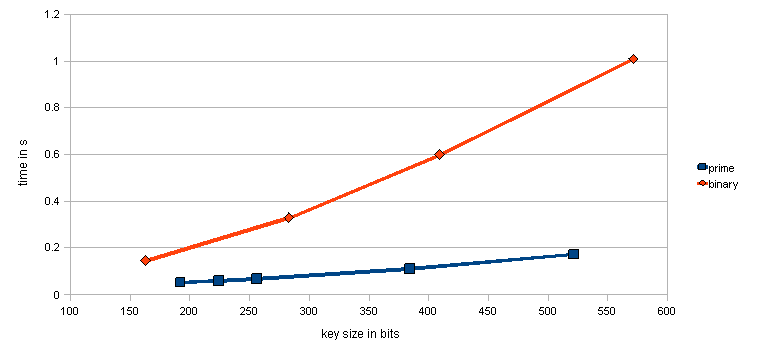
\includegraphics[scale=0.6]{keygen.png}
\caption{Key-pair generation, with prime and binary curves.}
\label{figure:keygen}
\end{figure}

As expected, the time increases about linearly with the key size, while the slope in prime curve is slightly higher than in binary curves.. The operation done is essentially one elliptic curve point multiplication. The timings for all tested curves don't exceed one second and are therefore feasible. The computation in prime curve show a significant advantage over the binary curves. The difference most likely comes from the fact that the binary curve arithmetic uses binary field arithmetic built from scratch while prime field arithmetic was done using GMP. For a definite result, more optimized binary field arithmetic should be used.

\subsection{Encryption and Decryption}
While in the key-generation test the processed data depends on the key-size, in the encryption and decryption test all cases process a file of the same size: 3.3KB. Because a curve with double key size can store the double amount of information on one point, larger key sizes have the theoretical advantage that less ciphertext-points are produced and therefore less operations are done. The results are illustrated in Figure \ref{figure:encdec}.

\label{encdecres}
\begin{figure}[h]
\centering
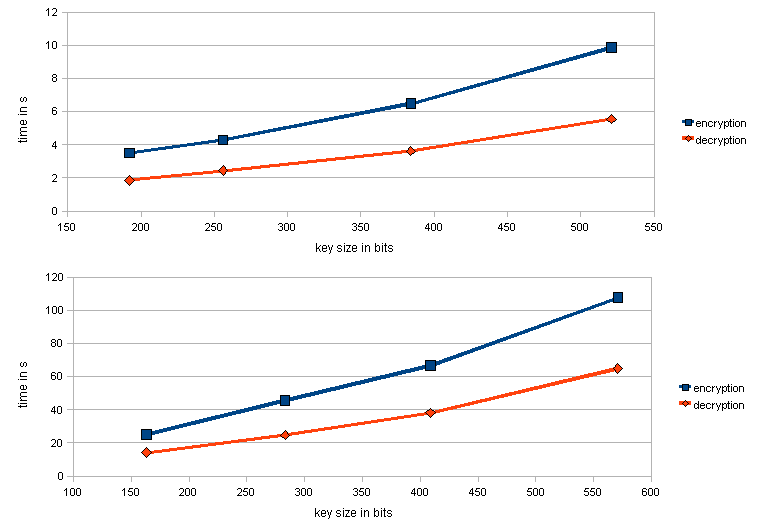
\includegraphics[scale=0.6]{dia2.png}
\caption{Encryption/Decryption results on a 3.3KB file}
\label{figure:encdec}
\end{figure}

The first thing we observe is that encryption takes approximately twice as much time as decryption. This is explained with the fact that encryption requires two multiplication while decryption needs only one (see Table \ref{elgoperations}). We again see a significant advantage of the prime curves like in curve generation. Furthermore it can be oversved that the efficiency of smaller keys is better than of larger keys, even though the total number of processed blocks is higher. The slope of the measurement curves is however steeper in key-generation.

As a general comment, public-key cryption is in practice not very often used for actual encryption because of its inferior performance compared to symmetric key cryptography. Instead it is usually used to establish a symmeteic key and the actual encryption is done for example with AES. We can also see in our results that the efficiency of our implementation is not sufficient to encrypt large files in a reasonable time.

\subsection{Point Counting with AGM}
The first attempt with the AGM algorithm was an implementation of the underlying polynomial multplication and reduction ``from scratch''. This was identified as the clear bottleneck as the runtime for a key-size of ~300 bits was about 30 minutes. We therefore decided replace this operations with the ones provided by the NTL library, which resulted in a dramatic performance improvement: the runtime for the same key-size was reduced to only a few seconds. The results are illustrated in Figure \ref{figure:agm}.

\label{agmres}
\begin{figure}[h]
\centering
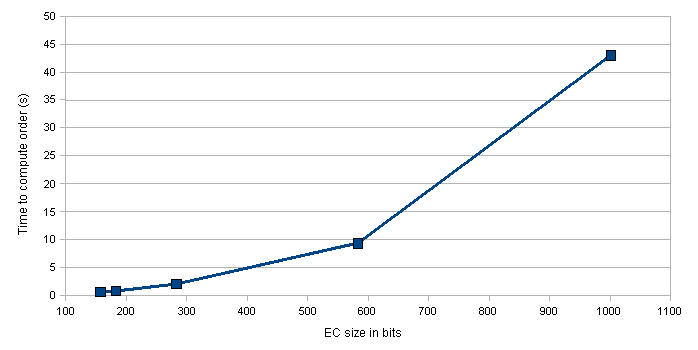
\includegraphics[scale=0.6]{dia1.png}
\caption{AGM point counting with varied key sizes.}
\label{figure:agm}
\end{figure}

The initial goal to be able to generate random curves in only a few seconds is achieved by looking at the results for key sizes up to about 500 bits. As an additional step for curve generation, an early-abort strategy to skip insecure curves \cite{satohfgh} would be needed. As described in the reference, a single point counting run dominates the early-abort step, from which we can conclude the feasiblilty of the AGM approach.

\subsection{Challenge Solution}
For testing the correctness of the implementation we were given a test consisting of the following tasks:

\begin{itemize}
 \item Generating an elliptic curve over prime field.
 \item Decrypting two messages over prime field.
 \item Decrypting two message over binary field.
 \item Deciding which message was forged.
\end{itemize}

In the first task, we were given the prime field modulus and some information needed to generate a curve using the complex muliplication method. The modulo equals the 13th mersenne prime ($n=2^{521}-1$), the imaginary field discriminant for complex multiplication is $D>-400$ and the EC parameter $a=-3$. The original description is available in Appendix \ref{appendixa}.

Finally the private key definition, readable by our implementation for the first curve was (for the format, see section \ref{ecdefinitions}):

\begin{verbatim}
 prime
6864797660130609714981900799081393217269435300143305409394463459185543183397656052 \
  122559640661454554977296311391480858037121987999716643812574028291115057151
-3
3527776260069785152007274377287143876629163004151083436918067245834023095352803352 \
  619592071776153064995010045981739923633622717991755444624957640186908953364
-398540598942556796715601841984589553814663412077882118326991138647122232976515044 \
  0620991823676837980440324457306600557245758586407123663426871114407190797434
6864797660130609714981900799081393217269435300143305409394463459185543183397650992 \
  549354694781534209408074441975667428948389124479097456824493161776014158579
2744834878295875502523990898255970938931750803137064564739517102097730423490652151 \
  435936560016891481734286491312379889015178748930010199888643781513
\end{verbatim}

And for the second curve:

\begin{verbatim}
 prime
6864797660130609714981900799081393217269435300143305409394463459185543183397656052 \
  122559640661454554977296311391480858037121987999716643812574028291115057151
-3
3527776260069785152007274377287143876629163004151083436918067245834023095352803352 \
  619592071776153064995010045981739923633622717991755444624957640186908953364
+277633783987862290745991157088307728706423274798898334066464657055442467551243242 \
  7452835254055623705198536338718514654123364891577242648186860775805757142087
6864797660130609714981900799081393217269435300143305409394463459185543183397650992 \
  549354694781534209408074441975667428948389124479097456824493161776014158579
1237946678497568790188826094418628206193474380513556414420549154032544215130643918 \
  215405913748994282110182353617745746987799819718799994745251376454
\end{verbatim}

The decrypted first ciphertext is (without new lines):

\begin{verbatim}
 f(z) : m = 283 in Table A.1, a = 1, b =
 43fdf8a39baa3eaad2fc71f1329184399a63e6fc51239c3df5e8b9e9de57618887eee7c, P =
 +587e2fa0ab7ccd194ba4d79aa859b109adef00bc75c66bf6c69a2536c256b8bb816927b. Private
 key = 26334010226743190633240527195230292831833139108096019898661304553382794977231705.
 Cypher : (+2996b532a62d94cd884558af3a22e4352e748808bab983bddbf387c35a4c0847a62d92c,
 -464089c5b600dfe844fcf0c9fbfb5056a8b166c70cdaf501b9ea59a0e1f8b3c0255e1ac)
 (-735bb3c6145270c85c8b4990fd76881fea861a2696f66074613a0ad088ae9ac829b1976,
 +d8d0ef69942277d300e3e1c8c679fc539f736cd1207ca536ff1156d0b50484b7f93cf8).
\end{verbatim}

The decrypted second ciphertext is:

\begin{verbatim}
 f(z) : m = 283 in Table A.1, a = 0, b =
 7cb16923a86f239ccb3d1cd7bd4d3de5dc3b97eda43330f533da57d8c208701899724dd, P = 
-fb4941d427a0b0ffe32ba899f6c8c7c9f89ad50f7291853d44004a5ea72762b048a54a. Private key =
 26326629228593706558136978105130308473615944643701116377878072489053032875983292312
8. Cypher : (-1c77506e381a30b83def3e1ebb8d835a49108ee89ad826e5342d5285a0e4f9cb1f0bd28,
 -1a48f416a4c3047701154062bfe56552e18bea284c6b3eff14d3f7ce30e311af61d27ee)
 (-7ba754244a3b5fd85c6f64a7d959fc24e5b766d383684886fe5171ca64b59eba09af9fe,
 -350c1b2efdb3bd7d3579158820c358c99328d329e6bce9f189937fab79019aa3e3797d8).
\end{verbatim}

So there is a second layer in the challenge, which consists of full definitions of two binary curves and two ciphertexts. The curve order isn't included, but not necessary for decryption. The reduction polynomial can be read from a table and is $z^{283}+z^{12}+z^7+z^5+1$. The first curve is defined as
\begin{displaymath}
 y^2 + xy = x^3 + x^2 + 43fdf8a39baa3eaad2fc71f1329184399a63e6fc51239c3df5e8b9e9de57618887eee7c
\end{displaymath}
and the second as 
\begin{displaymath}
 y^2 + xy = x^3 + 7cb16923a86f239ccb3d1cd7bd4d3de5dc3b97eda43330f533da57d8c208701899724dd
\end{displaymath}

Afer bringing this information in the format readable for our application, the ciphertext was decrypted. The first message is:

\begin{verbatim}
 Class number for discriminant -877991 equals 818.
\end{verbatim}

The decrypted second message is:

\begin{verbatim}
 Class number for discriminant -1293367 equals 513.
\end{verbatim}

The class number is a well-known invariant in Algebraic Number Theory and can be computed using standard algebra libraries. Using the sage library, it was found that the first solution is true while the other is false (the class number in the second case is 511). Hence, the second message was forged.

\section{User Guide}
This section is intended to provide information to the interested user who wants to experiment with our application.
With the command line interface, our program provides a convinient way to use elliptic curve cryptography in practice. The functionalities, and how they are used is presented, along with some practical examples.

\subsection{Getting the Source}
The program source itself can be downloaded over one of the two identical repositories: \url{http://github.com/gadial/ECC} and \url{http://github.com/bhess/ECC}. One can also use git to download the source:
\begin{verbatim}
 #> git clone git://github.com/gadial/ECC.git
\end{verbatim}
Once the repository is cloned, the source can be actualized with
\begin{verbatim}
 #> git pull
\end{verbatim}
\emph{git} itself is available under \url{http://git-scm.com}.

\subsection{Compiling the Source}
The source repository provides a makefile, so that the source is compiled by running
\begin{verbatim}
 #ECC> make
\end{verbatim}
in the root folder.

\subsubsection{Dependencies}
In order to successfully compile the source, some shared libraries should be installed. We recommend to install current versions of the following libraries (in braces are tested versions):

\begin{itemize}
 \item CppUnit (version 1.12.0) \url{http://cppunit.sourceforge.net}
 \item GMP - GNU Multi-Precision Library (version 4.3.1) \url{http://gmplib.org}
 \item NTL (version 5.5.2) \url{http://www.shoup.net/ntl}
\end{itemize}

The program is tested under 32 bit Linux, as compiler g++ version 4.4.1 was used.

\subsection{Elliptic Curve Definitions}
\label{ecdefinitions}
Public-key and private-keys contain the full definition of the corresponding elliptic curve. The files must be provided to the application in order to do encryption and decryption. A sample public-key file looks as following:

The format is the following:

\begin{itemize}
 \item 1. line: ``prime'' or ``binary'' curve.
 \item 2. line: Elliptic curve modulus (prime) or reduction polynomial (binary)
 \item 3. line: Parameter $a$.
 \item 4. line: Parameter $b$.
 \item 5. line: Point $P$ on the elliptic curve, in compressed form.
 \item 6. line: Elliptic curve order.
 \item 7. line: Public key (in compressed form) or private key.
\end{itemize}

All values must be decimal. A sample public key definition for a prime curve could look the following way:

\begin{verbatim}
prime
6277101735386680763835789423207666416083908700390324961279
-3
2455155546008943817740293915197451784769108058161191238065
+602046282375688656758213480587526111916698976636884684818
6277101735386680763835789423176059013767194773182842284081
-4202774374097843812550356794057673546542297328739257456130
\end{verbatim}


\subsection{Command Line Interface}
Over a simple command line interface, the following three concepual functions of the cryptosystem can be used:
\begin{itemize}
 \item Key-pair generation.
 \item Encryption
 \item Decryption
\end{itemize}

When the executable is run without switch, the usage parameters are displayed:

\begin{verbatim}
 #ECC> ./ECC
Usage:
ECC {-pk </path/to/pk> -enc </path/to/plaintext> |
     -sk </path/to/sk> -dec </path/to/ciphertext> |
     -gen_key {-ec_name 'name' | -use_ec </path/to/ec>}
     -validate </path/to/ec>
Predefined Curves (NIST): [p192|p224|p256|p384|p521|b163|b283|b409|b571]
\end{verbatim}

\subsubsection{Key-pair Generation}
By using the switch \emph{-gen\_key} we indicate that a public-key/private-key should be generated. For this purpose the elliptic curve has to be known. The 9 curves recommended by NIST are built-in and can be specified with the switch \emph{-ec\_name}. In the NIST curve names, 'p' indicates a prime curve and 'b' a binary curve; the number afterwards indicate their bit-size. If we want to generate a key-pair with the curve \emph{p192}, we run:

\begin{verbatim}
 #ECC> ./ECC -gen_key -ec_name p192
\end{verbatim}

Then two textfiles, containing the curve information and the keys are generated (the file-names contain a timestamp when the curve key has been generated):

\begin{verbatim}
 #ECC> cat public_key_201003220104.txt
prime
6277101735386680763835789423207666416083908700390324961279
-3
2455155546008943817740293915197451784769108058161191238065
+602046282375688656758213480587526111916698976636884684818
6277101735386680763835789423176059013767194773182842284081
-4202774374097843812550356794057673546542297328739257456130
\end{verbatim}

\begin{verbatim}
 #ECC> cat private_key_201003220104.txt
prime
6277101735386680763835789423207666416083908700390324961279
-3
2455155546008943817740293915197451784769108058161191238065
+602046282375688656758213480587526111916698976636884684818
6277101735386680763835789423176059013767194773182842284081
3693200230270282832430567472370334031293814885720270459444
\end{verbatim}

The second possibility is to use a curve-definition from a file. In the next example, we take the above generated public-key file as definition of a curve.

\begin{verbatim}
 #ECC> ./ECC -gen_key -use_ec public_key_201003220104.txt
\end{verbatim}

And the following files are created:

\begin{verbatim}
 #ECC> cat public_key_201003220109.txt
prime
6277101735386680763835789423207666416083908700390324961279
-3
2455155546008943817740293915197451784769108058161191238065
+602046282375688656758213480587526111916698976636884684818
6277101735386680763835789423176059013767194773182842284081
+6073060550633047313222863878319194062684276429882449125142
\end{verbatim}
\begin{verbatim}
 #ECC> cat private_key_201003220109.txt
prime
6277101735386680763835789423207666416083908700390324961279
-3
2455155546008943817740293915197451784769108058161191238065
+602046282375688656758213480587526111916698976636884684818
6277101735386680763835789423176059013767194773182842284081
4495925941769958181740011055363126307352799406048087058490
\end{verbatim}

A function to generate a random curve directly over the command line is currently not available. For random curve generation, the program API has to be used directly.

\subsubsection{Encryption}
For encrypting textfiles, one needs to provide a public-key file which also contains the elliptic curve definition. Suppose we want to encrypt the file \emph{faust.txt}:

\begin{verbatim}
 #ECC> cat faust.txt
Habe nun ach! Philosophie, Juristerei und Medizin, und leider auch Theologie!
durchaus studiert mit heissem Bemuehn. Da steh ich nun, ich armer Tor! und bin so
klug als wie zuvor; heisse Magister, heisse Doktor gar, und ziehe schon an der zehen
Jahr herauf, herab und quer und krumm meine Schueler an der Nase herum - und sehe,
dass wir nichts wissen koennen! Das will mir schier das Herz verbrennen!
\end{verbatim}

We use the first public-key generated in the last section with the NIST curve p192 for encryption, and the command is:

\begin{verbatim}
 #ECC> ./ECC -pk public_key_201003220104.txt -enc faust.txt
\end{verbatim}

The name of the file containing the ciphertext is the plaintext-name with extension \emph{.enc}. The ciphertext point-pairs are written in compressed form and are separated line by line (in the following some contents were truncated for layout reasons):

\begin{verbatim}
 #ECC> cat faust.txt.enc
-2941418657115936641805...,+1926840320549465382934...
+1538291260063052821414...,+4260644256050139287355...
-2348564039062829639347...,+2883638826011508920689...
+4677737476484516605321...,+3559085594982234746243...
+7134535296842259156817...,-3305284033086540132053...
-3357881763927395711480...,-5323445310157508381249...
+5981876371431035768184...,-5576058672905230562784...
...
...
\end{verbatim}

\subsubsection{Decryption}
Analogue to encryption, we provide the private key containing the curve definition to the command line interface to decrypt a ciphertext. To decrypt the example from before, run the following:

\begin{verbatim}
 #ECC> ./ECC -sk private_key_201003220104.txt -dec faust.txt.enc
\end{verbatim}

The decrypted file has the file-extension \emph{.dec}, and indeed, the decryption was successful:

\begin{verbatim}
 #ECC> cat faust.txt.enc.dec
Habe nun ach! Philosophie, Juristerei und Medizin, und leider auch Theologie!
durchaus studiert mit heissem Bemuehn. Da steh ich nun, ich armer Tor! und bin so
klug als wie zuvor; heisse Magister, heisse Doktor gar, und ziehe schon an der zehen
Jahr herauf, herab und quer und krumm meine Schueler an der Nase herum - und sehe,
dass wir nichts wissen koennen! Das will mir schier das Herz verbrennen!
\end{verbatim}

\subsubsection{Elliptic Curve Validation}
For elliptic curves defined in a text-file, the switch -validate provides a quick and handy function to validate that the provided parameters are correct. Beside curve definition files consisting of 6 lines, also private and public keys can be provided, where the last line defining the key is simply ignored.

Suppose we wanto to validate the elliptic curve defined in the following public-key file:

\begin{verbatim}
 #ECC> cat ./challenge/private_key_binary1.txt
binary
15541351137805832567355695254588151253139254712417116170014499277911234281641667989665
1
8255380585809383688639434939783260988279527409588319652248090673203645932948626009724
+10744526979748405769424843092044115614633826679604470999470890953483892379364112110203
15541351137805832567355695254588151253139256032115589896844343002557484362928298853438
26334010226743190633240527195230292831833139108096019898661304553382794977231705
\end{verbatim}

To validate we run:

\begin{verbatim}
 #ECC> ./ECC -validate ./challenge/private_key_binary1.txt
Validation succeeded!
\end{verbatim}

More specifically, the test reads in the EC parameters, uncompresses the point on the curve and multiplies the point with the curve order. If the result is the point at infinity, the validation succeeds and otherwise it failes.

\subsubsection{Testcases}
The implementation has a big number some built-in testcases that test different aspects of the implementation, like finite field arithmetic or several algorithms. With the switch -t the testcases are launched:
\begin{verbatim}
 #ECC> ./ECC -t
 .....................................................

 OK (53)
\end{verbatim}
This is mainly for debugging purposes and shows that ``everything should be right'', especially after changes in the code are made.

\section{Conclusion}
In this project we investigated the large field of elliptic curve cryptography, whose properties enable to achieve the same security with much smaller key sizes compared to public key cryptography over $\mathbb{Z}_n^*$. We implemented an elliptic curve cryptosystem ``from scratch'', relying only on big integer arithmetic. This implied the implementation of finite field arithmetic and several additional algorithms. Furthermore, the implementation was done for both elliptic curves over prime and binary fields. Besides the deep insight this approach gave, also some limitations were shown, namely not all our implementation can compete with highly optimized libraries.

Besides the cryptosystem, we implemented two cutting-edge methods to generate random elliptic curves. The two approaches are conceptually different: the \emph{Complex Multiplication} (over prime fields) generates a curve for a given order, and the \emph{AGM} point-counting method (over binary fields) computes the order for given curve parameters. We showed the practical feasibility of both methods and that a random curve with not too large bit-size up to about 300 bits can be generated within a few seconds. We sucsessfully solved a challenge consisting of generation of a prime curve, and decryption over a prime and a binary curve. 

Further work could involve the implementation of Complex Multiplication for binary fields and point-counting for prime fields, which would enable a direct comparison between binary and prime curves. Several optimizations could be done, either by choosing more efficient algorithms or by low-level optimizations. Additionally, a comparison of our implementations with variants from optimized library would be interesting. As cryptosystem, we choose the ECC ElGamal system for encryption and decryption. An additional task would be to implement a signature scheme, or to choose a different encryption system.

For end-users, the product of our project is an elliptic-curve-cryptosystem that is ready-to-use. One can either define own curves or choose between different predefined curves recommended by NIST, which are then used for key-generation, encryption, and decryption of arbitrary text-messages. The entire implementation in C++ consists of approximately 7500 lines of code.

\begin{appendix}
\section{Challenge Description}
\label{appendixa}
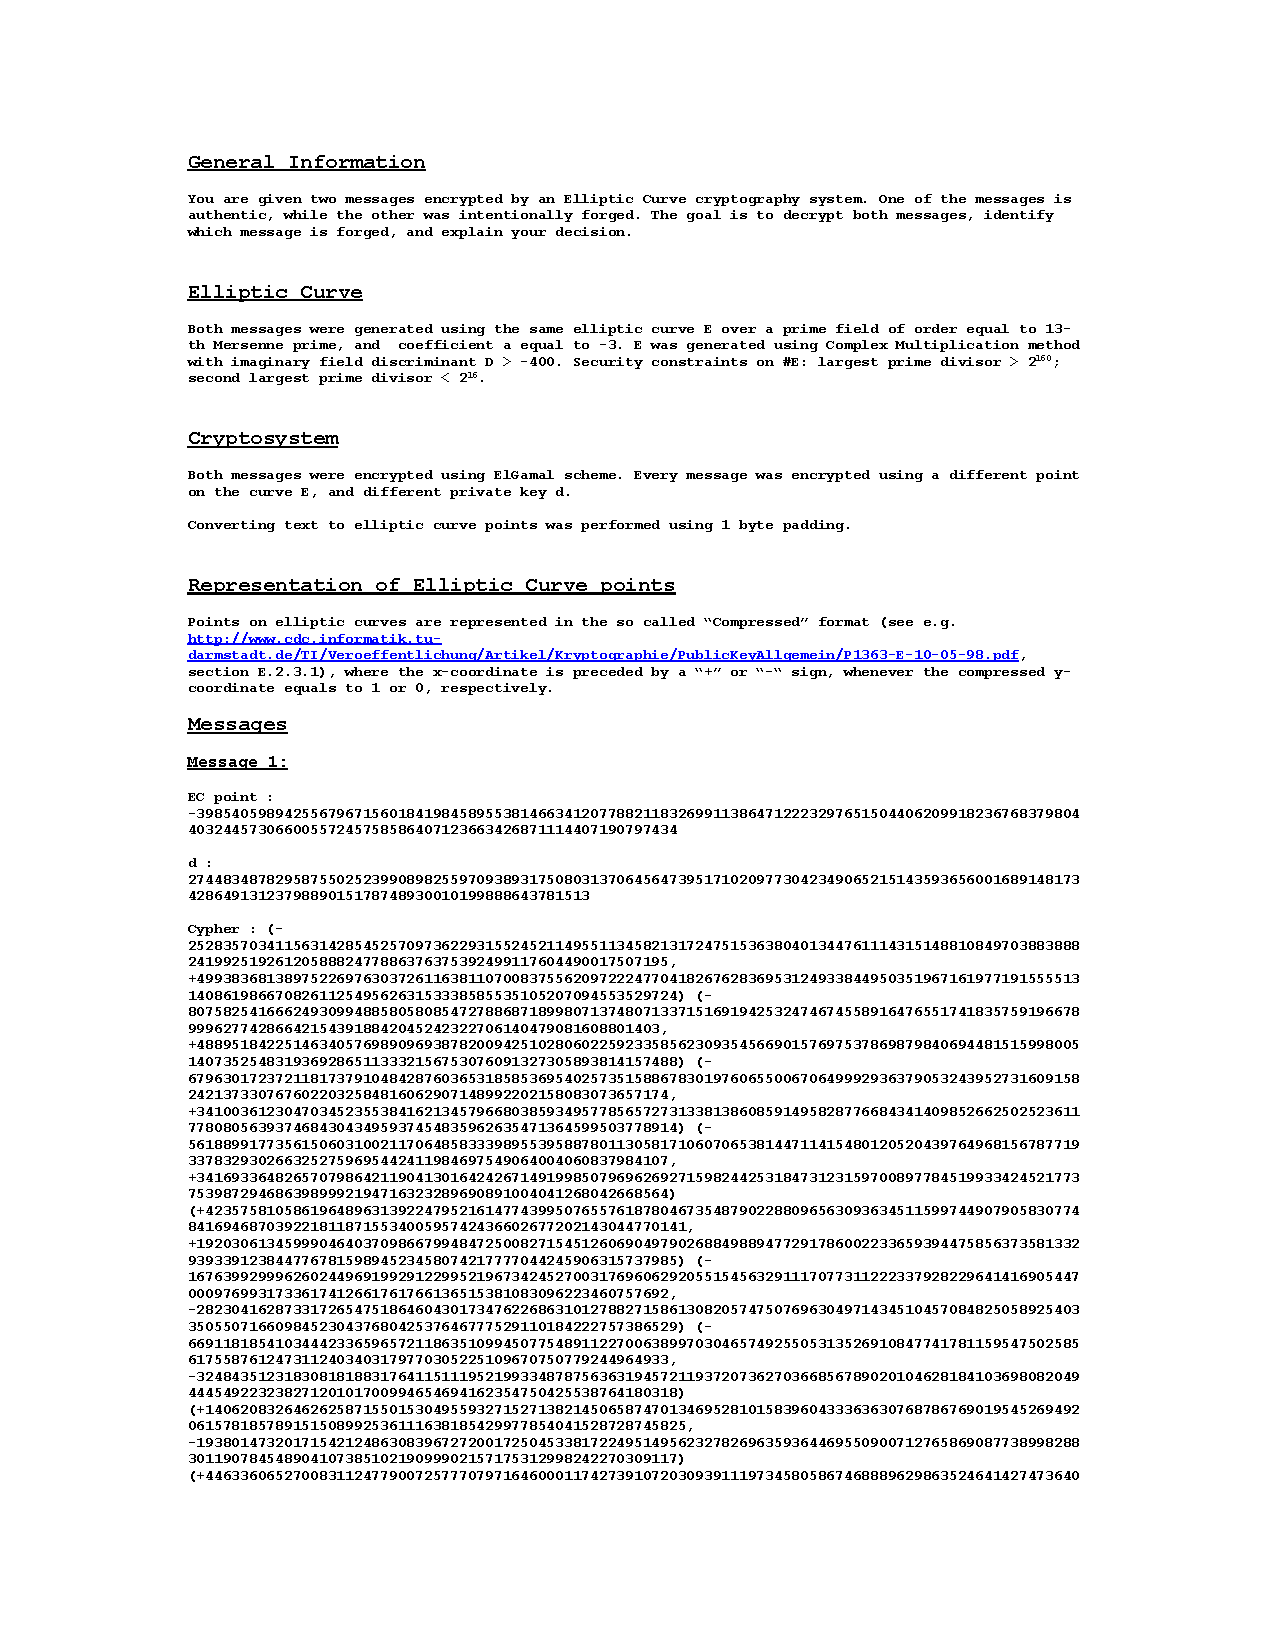
\includepdf[pages=1-2]{236349_Project_Test_2009.pdf}
\end{appendix}

\newpage
\bibliographystyle{plain}
\bibliography{eccbib}
\end{document}
